% intro.tex:

\chapter{Introduction}
\label{chap:intro}
This is where the intro goes.
There is a planet ... where people still believe digital watches are the
greatest invention. It is mostly harmless.

\section{Life, Universe and Everything}
\label{chap:intro:design}

Simple, quantitative answers to the most pondering questions are beautiful. More about question of life, universe and everything can be found in \cite{book:42}.

This is where the text goes. One can refer to a previous chapter like \chapref{chap:intro}. To find all the other reference possibilities search in the MACROS folder for chapref. Also one can include pictures, preferably in the pdf format like shown in \figref{fig:intro:meth}. Graphics can also be included as eps, if graphics is in eps, the epstopdf packages converts it to pdf on the fly. See examples below in \figref{fig:intro:meth2}.

To keep the code clean, call all extra packages that you would like to use from the file macro.tex in the macro folder. Also keep all your graphics in the fig folder and all bibliography related files in the bib folder.

Make sure that you run bibtex and makeindex to geberate bibliography and index.

This demonstrates how to include a term\index{Term} into the index\index{Index}. For details, check out \cite{latex:index}.

\begin{figure}[htbp]
  \centering
    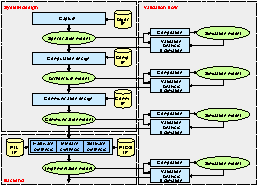
\includegraphics[width=0.5\textwidth]{fig/meth.pdf}
  \caption[Design methodology for SoC design]{\label{fig:intro:meth} Design methodology for SoC design (Source \cite{book:SpecC:yellow})}
\end{figure}

\begin{figure}[htbp]
  \centering
    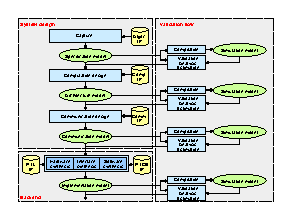
\includegraphics[width=0.5\textwidth]{fig/meth.eps}
  \caption{\label{fig:intro:meth2} Design methodology but included as EPS figure}
\end{figure}

Also tables are possible as shown in \tabref{tab:ConclusionSummary}. What is really cool are the acronyms. The first time you use one, like \ac{TLM} then it appears with full description. Using it the second time makes only the acronym appears \ac{TLM}.

\begin{table}[htbp]
  \centering
     \begin{tabular}{|l|c|}
        \hline
         \textbf{Environment Condition} & \textbf{Applicable Model} \\
			\hline
			 \begin{tabular}{@{}l@{}}
			 $\bullet\,$ single master bus \\
			 $\bullet\,$ no overlap between masters bus access\\
			 \end{tabular}
			&
			 \ac{TLM}
			\\
			\hline
			 \begin{tabular}{@{}l@{}}
			 $\bullet\,$ only locked transfers \\
			 $\bullet\,$ unlocked transfers and low overlap\\
			 \end{tabular}
			&
			 \ac{ATLM}
			\\
			\hline
			 \begin{tabular}{@{}l@{}}
			 $\bullet\,$ unlocked transfers and high overlap\\
			 \end{tabular}
			&
			 bus functional
			\\
			\hline
		\end{tabular}
	\caption{Conclusion summary}
	\label{tab:ConclusionSummary}
\end{table}

Now time for some math\index{Math}:
\begin{align}
F(x)&=\int_{-\infty}^x f(u)\,du\\
\bm{Ax}&=\bm{b}\\
\mathbf{Ax}&=\mathbf{b}\\
\sin^2(\theta)+\cos^2(\theta)&=1\\
x&\in\mathcal{X}
\end{align}

The difference in using \verb1\bm1  and \verb1\mathbf1  is clear from above.
% --- EOF ---
